\chapter{Исследовательский раздел}
\label{cha:research}

Программное обеспечение было реализовано на дистрибутиве Ubuntu 20.04, ядро версии 5.19.0.

\section{Пример работы разработанного программного обеспечения}

Пусть содержимое рассматриваемой директории имеет вид, изображенный на рисунке \ref{fig:ls_before}.

\begin{figure}[ph!]
	\center{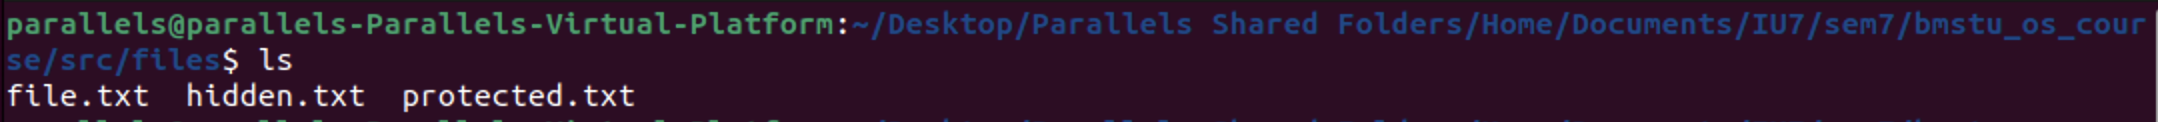
\includegraphics[scale=0.43]{img/ls_before.png}}
	\caption{Содержимое папки до загрузки модуля}
	\label{fig:ls_before}
\end{figure}

Файлы, содержащие списки контроля доступа, находятся в директории /proc.
На рисунке \ref{fig:proc} изображен пример формирования таких списков. 

\begin{figure}[ph!]
	\center{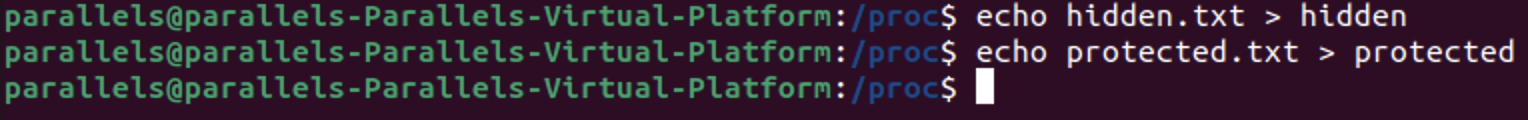
\includegraphics[scale=0.6]{img/proc.png}}
	\caption{Создание файлов, содержащих списки контроля доступа}
	\label{fig:proc}
\end{figure}

Файл hidden содержит имена файлов, которые необходимо скрыть полностью, файл protected ---  имена файлов, которые нельзя открывать, изменять, удалять.

После загрузки модуля содержимое рассматриваемой директории выглядит следующим образом (рисунок \ref{fig:ls_after}).

\begin{figure}[ph!]
	\center{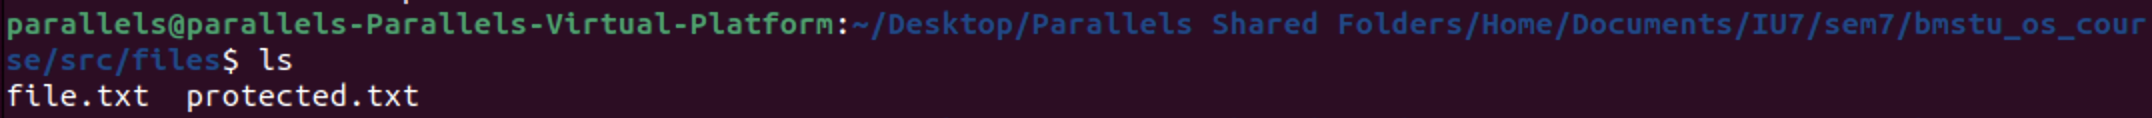
\includegraphics[scale=0.43]{img/ls_after.png}}
	\caption{Содержимое папки после загрузки модуля}
	\label{fig:ls_after}
\end{figure}

Результат выполнения команды ls не содержит файл hidden.txt.

После ввода пароля (рисунок \ref{fig:pass1}) файл hidden.txt перестает быть скрытым (рисунок \ref{fig:pass_after1}).

\clearpage

\begin{figure}[ph!]
	\center{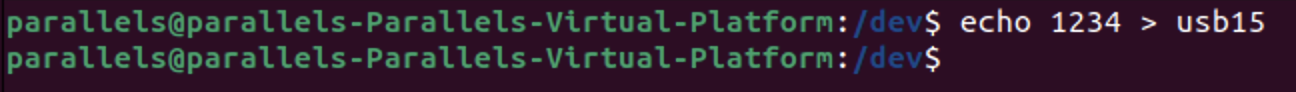
\includegraphics[scale=0.53]{img/pass1.png}}
	\caption{Ввод пароля}
	\label{fig:pass1}
\end{figure}


\begin{figure}[ph!]
	\center{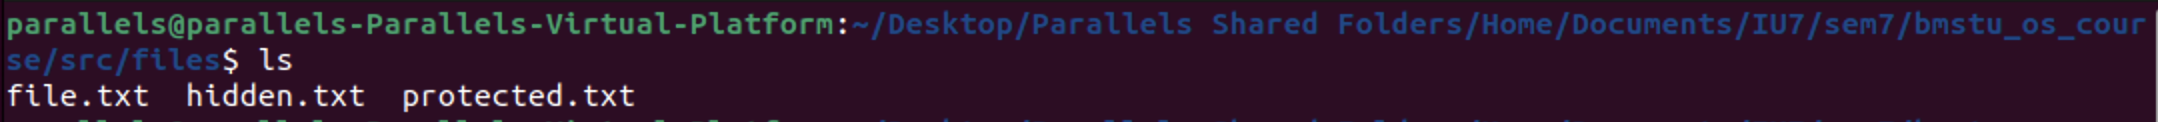
\includegraphics[scale=0.43]{img/ls_before.png}}
	\caption{Результат работы команды ls после ввода пароля}
	\label{fig:pass_after1}
\end{figure}

При попытке удалить файл protected.txt (рисунок \ref{fig:rm}) или вывести его содержимое с помощью cat ничего не происходит.

\begin{figure}[ph!]
	\center{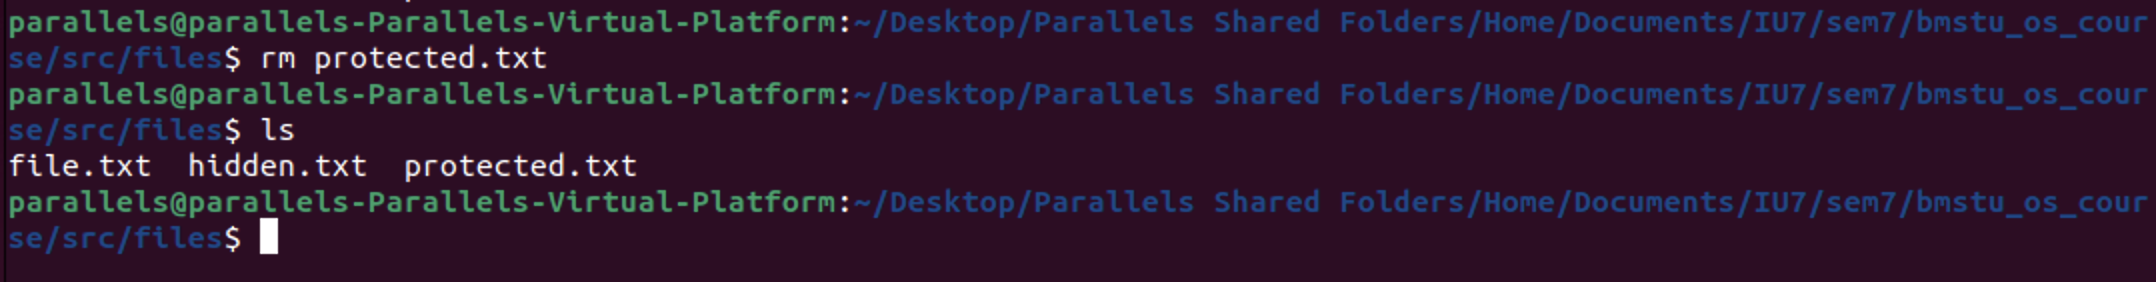
\includegraphics[scale=0.45]{img/rm.png}}
	\caption{Удаление файла protected.txt}
	\label{fig:rm}
\end{figure}

\begin{figure}[ph!]
	\center{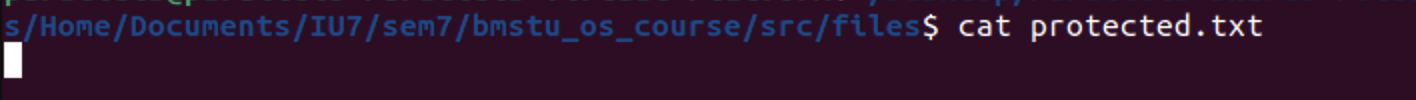
\includegraphics[scale=0.6]{img/cat.png}}
	\caption{Вывод содержимого файла protected.txt}
	\label{fig:cat1}
\end{figure}

После ввода пароля (рисунок \ref{fig:pass2}) операции над файлом protected.txt становятся возможными (рисунок \ref{fig:cat2}).

\begin{figure}[ph!]
	\center{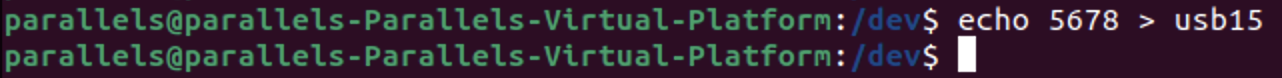
\includegraphics[scale=0.6]{img/pass2.png}}
	\caption{Ввод пароля}
	\label{fig:pass2}
\end{figure}

\begin{figure}[ph!]
	\center{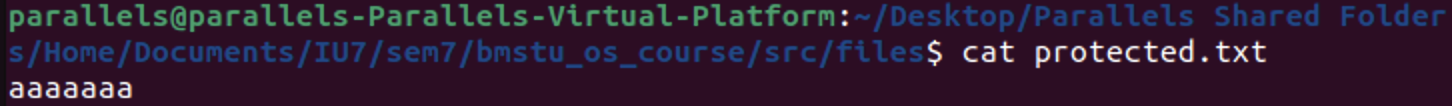
\includegraphics[scale=0.6]{img/cat_work.png}}
	\caption{Вывод содержимого файла protected.txt после ввода пароля}
	\label{fig:cat2}
\end{figure}


